\documentclass{article}

\usepackage[utf8]{inputenc}
\usepackage[T1]{fontenc}

\usepackage{a4wide}

\usepackage{amsmath}
\usepackage{amssymb}
\usepackage{amsthm}

\usepackage{hyperref}

\usepackage{graphicx}

\title{Swarm intelligence: Ant colony optimization project}
\author{Samuel Buchet: 000447808}
\date{June 2017}

\begin{document}

\maketitle

\section*{Introduction}

In this project, two ant colony optimization algorithms are implemented to solve the Closest String Problem.
The two algorithms implemented are the Max Min Ant System algorithm (MMAS) and the Ant Colony System algorithm (ACS).
In the following report, the two algorithms are first described.
After that, the two algorithms are compared.
Finally, a local search is used to improve the results.

\section{Implementation of the algorithms}

In this section, the Max Min Ant System and the Ant Colony System algorithms are described.
These two agorithms also use a heuristic information which is explained below.

\subsection{Heuristic information}

In \cite{aco_csp}, no heuristic information is used.
However, most of the ant colony algorithms use this kind of information.
In addition, it can be easily computed for a lot of problems.
It has been decided to define one for the closest string problem. \newline

The goal of the closest string problem is to minimize the maximum hamming distance between the solution and the set of strings.
To minimize the distance between the solution and the set of strings, a greedy decision consists in adding into the solution the character which appears the most in the set of strings at a given position.
Indeed, by using this character, the distance might be equal to 0 at this position.
For each character at each position of the string, a greedy score can be defined as the frequency of the character.\newline

However, the frequencies might be very close to each other.
As a result, if this score is used in the probabilities, the probabilities of getting the best greedy character would be very low.
To solve this problem, the exponential function is applied to the score after scaling it.
The final score of character $j$ at position $i$ is equal to: $score_{ij} = \frac{exp(5*frequency_{ij})*1.5}{max_j(frequency_{ij})}$ where $frequency_{ij}$ is the number of occurences of the character $j$ at position $i$ in the set of string of the problems.
The parameters have been chosen after testing different values.

\subsection{Basic ant system algorithm}

Both variants of the ant colony algorithms implemented in this project rely on the same basis.
At each iteration, the general algorithm builds $n$ solutions (with $n$ equal to the size of the population) and then updates the pheromones with the formula: $\tau_{ij}(t) = (1-\rho)*\tau(t-1) + \sum \limits_{k=1}^m \Delta \tau_{ij}^k$  where $\tau_{ij}(t)$ is the amount of pheromone at position $i$ for character $j$ after t iterations, $\rho$ is the evaporation rate and $\tau_{ij}^k$ is the quantity of pheromone deposited by ant $k$ if this ant have chosen character $j$ at position $i$. \newline

As seen in \cite{aco_csp}, the amount of pheromone deposited by the ants is equal to $1-\frac{HD}{m}$ where HD is the maximum hamming distance of the ant and $m$ is the length of the strings of the problem.
This quantity has been used in the two implementations of this project. \newline

To build a solution, each character is chosen according to a probabilty.
The probability of choosing the character $j$ at position $i$ is equal to $ \frac{greedyScore_{ij}^{\alpha} * \tau_{ij}^{\beta}}{\sum probas}$ where $greedyScore$ is the greedy score described previously and $\tau_{ij}$ is the amount of pheromone at position $i$ for the character $j$.


\subsection{Max Min Ant System}

In the Min Max Ant System algorithm, the pheromones are constrained with an upper and a lower bound.
At the begining of the algorithm, the pheromones are initialised to $+\infty$.
After each pheromone updates, the pheromones are checked.
If it exeeds the lower or the upper bound, the pheromone is re-assigned to this bound. \newline

In this implementation, the upper bound is equal to $1-\rho*\frac{D_{best}}{m}$ where $D_{best}$ is the value of the best solution found so far and $m$ is the length of the string.
The lower bound of the pheromones is equal to $\frac{up}{a}$ where $up$ is the upper bound and a is a parameter.
These two bound are updated each time a better solution is found.\newline

In this Max Min Ant System implementation, the best solution of a population generation is the only one which deposits pheromones.
An addition component is used to prevent the algorithm from converging.
If a convergence is detected, the pheromones are re-initialised to the upper bound.
The convergence is detected by a certain number of iterations without any improvements of the best solution found.
This number of iterations is equal to $iterations*convRate$ where $iterations$ is the maximum number of iterations allowed to the algorithm and $convRate$ is a parameter, between $0$ and $1$ which determines the percentage of the total time allowed to wait before pheromones re-initialisation.

\subsection{Ant Colony System}

The Ant Colony System algorithm is usefull to control the trade off between exploration and intensification.
In this variant, a additional rule is can be used to build a solution.
With probability $q_0$, the artificial ant chooses the character $j$ at position $i$ which maximizes $\tau_{ij}*\eta_{ij}^{\beta}$, where $\tau_{ij}$ is the amount of pheromones at position $i$ for the character $j$, $\eta_{ij}$ is the heuristic information for the same character and $q_0$ is a new parameter of the algorithm.
With probability $1-q_0$, the previous rule is applied (biased exploration).\newline

The pheromones update, which takes place after building the solutions of the population, is also modified.
Only the best ant so far deposits pheromones.
The amount of pheromones deposited is the same as before, but it is multiplied by the parameter $\rho$.
To finish, a new local update rule of the pheromones is used to introduce diversification.
During the construction of the solutions, for each decision chosen by the ants, the pheromones corresponding to that decision is updated as following: $\tau_{ij}=(1-\rho)*\tau_{ij}+\rho*\tau_0$, where $\tau_{ij}$ is the amount of pheromones for this decision and $\tau_0$ is the initial amount of pheromones.

\section{Parameter settings}

Parameter settings is a crucial step.
The ant colony optimization algorithms contain a lot of parameters and they are efficient only for a narrow range of values. \newline

\subsection{Process}

To make the tuning easier, the assumption that the parameters are not completely dependent is made.
This means that if a value which gives very good solutions is found for a parameter, the solution qualities will not change a lot by slightly modifying the other parameters.
With this assumption, a good setting can be found by modifying one parameter at a time.
If a significant improvement is found with a certain parameter, the other parameters can be re-tuned to continue improving the algorithm.
This process can be repeated with multiple instances until no significant changes are found anymore.\newline

To tune the parameters, it is also possible to display the informations of the algorithm during the execution of some instances.
For example, during the tuning phase of the algorihtms, the best solution found so far was displayed each time a better solution was found.
By doing this, it is possible to detect if the algorithm converges and if the total budget is used.
If no improvement occurs long before the end of the execution, this could mean that the algorithm has converged.
It can be checked by displaying the pheromones and it can be resolved by changing the $\rho$ value.\newline

To analyse the performance of the tuning, the solution returned by the algorithm can also be compared to a greedy solution.
The greedy solution can be generated by taking the character which maximizes the heuristic score described in section 1.
If the result of the ant colony algorithm is not better than the result of the greedy one, it could mean that the ant colony algorithm completely rely on the heuristic information and that the $\alpha$ and $\beta$ parameters should be modified.

\subsection{Max Min settings}

The number of ants has been set to $10$ in this algorithm, as done in \cite{aco_csp}.
With the same number of iterations, a higher value could give better results but it would require more evaluations.
The $\rho$ parameter should seem to be high comparing to \cite{aco_csp} (0.03).
However, the pheromones bounds and the pheromone re-initialisation prevent the algorithm form converging.
In order to properly use the pheromones, the $a$ parameter should be quite high.
However, higher values did not give better results, which can be caused by the very low value of the upper bound.
To finish, the $convRate$ parameter (percentage of the maximum number of iterations to wait before) has been adapted to keep enough time for intensification.\newline

\begin{tabular}{c|c}
    Parameter & Value \\ \hline
    $ants$    & 10    \\
    $\alpha$  & 1.8   \\
    $\beta$   & 2     \\
    $\rho$    & 0.12  \\
    $a$       & 60    \\
    $convRate$& 0.16  \\
\end{tabular}

\subsection{Ant Colony System settings}

In this algorithm, the number of ants is the same as before.
We can see that the value of $\rho$ is very low compared to the previous settings.
This can be explained by the fact that there is no bounds on the pheromones and no re-initialisation.
The initial amount of pheromone is also very low compared to the previous one ($+\infty$ for the max min ant system).
This value can be related to the percentage of the initial pheromone value deposited by all the ants during the construction of the solutions.
Finally, the $q_0$ parameter is greater than $0.5$ which means that the intensification rule is chosen more often. \newline

\begin{tabular}{c|c}
    Parameter        & Value \\ \hline
    $ants$           & 10    \\
    $\alpha$         & 1.2   \\
    $\beta$          & 2.5   \\
    $\rho$           & 0.015 \\
    $q_0$            & 0.6   \\
    $initPheromones$ & 0.026 \\
\end{tabular}

\section{Comparison of the algorithms}

To compare the algorithms, the relative percentage deviation has been computed with the mean of the 10 executions of each algorithm on each instance.

\subsection{Relative Precentage Deviations}

The table bellow shows the min, the max, the mean and the standard deviation of the relative percentage deviations.

As we can see, the value for the Min Max algorithm is always lower than the value of the Ant Colony System algorithm. \newline

To conclude that there is a statistically significant difference between the two algorithms, we can perform a Wilcoxon rank-sum test.
The test performed with a significance level equal to $0.05$ returns a p-value equal to $0.154$.
The p-value is greater than the significance level, which means that the null hypothesis is not rejected.
Thus, we cannot conclude that there is a statistically significant difference between the rpd of the two algorithms.
There is no algorithm which is statistically better than the other one.
However, regarding the results on the table bellow, we could recommend the Max Min algorithm, without any guarantee.

\subsection{Correlation of the rpd's}

The plot \ref{fig:corr} shows the correlation between the rpd's of the two algorithms for all instances.
Each color corresponds to the instances with a same number of characters in the alphabet. \newline

\begin{figure}
    \centering
        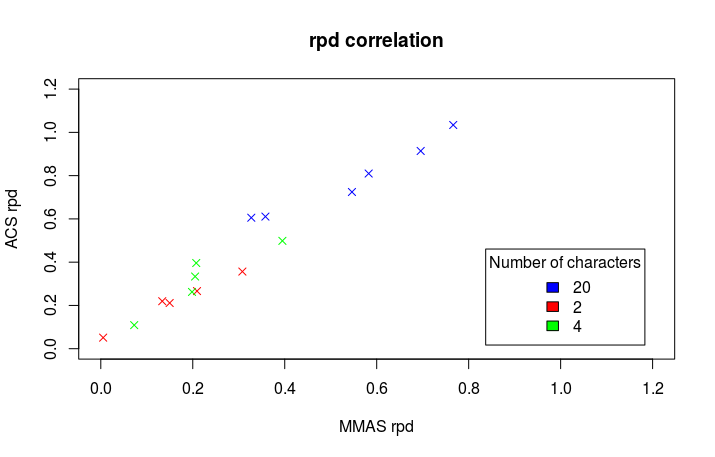
\includegraphics[scale=0.5]{correl}
    \caption{Correlation plot between the arpd's}
    \label{fig:corr}
\end{figure}

We can see that the rpd's of the rwo algorithms are correlated.
This can be confirmed with a spearman test.
With a significance level equal to $0.05$, the test returns a p-value equal to $8.085*10^{-6}$ which means that the results are correlated.
We can see on the graph that the instances with 20 characters are the most difficult.
The correlation shows that the more an instance is difficult for one algorithm, the more this instance will be difficult for the second algorithm.
This observation sows that the algorithm have a similar behaviour on the problem.

\subsection{Convergences of the algorithms}

The two plots \ref{fig:conv1} and \ref{fig:conv2} can be used to compare the convergence of the two algorithms.
These plots have been done using the same tuning with a number of iterations equal to 2000 to have enough time to observe the convergence.\newline

On both plots, we can see that the the Max Min algorithm is able to reach a better solution.
However, on the first plot, we can see that at the begining of the run, the Ant Colony System algorithm find better solutions than Max Min Ant System.
This result is not clear on the second plot but it could mean that for some instances, if the budget is very limited, it would be preferable to use the Ant Colony System Algorithm. \newline

On the first plot, we can see that the convergence of Ant Colony System is faster, which can be explained by the fact that it does not have a pheromone re-initialisation process like Max Min Ant System.
However, on the second plot, we can see that the convergence of the Ant Colony System algorithm is slower.

\begin{figure}
    \centering
        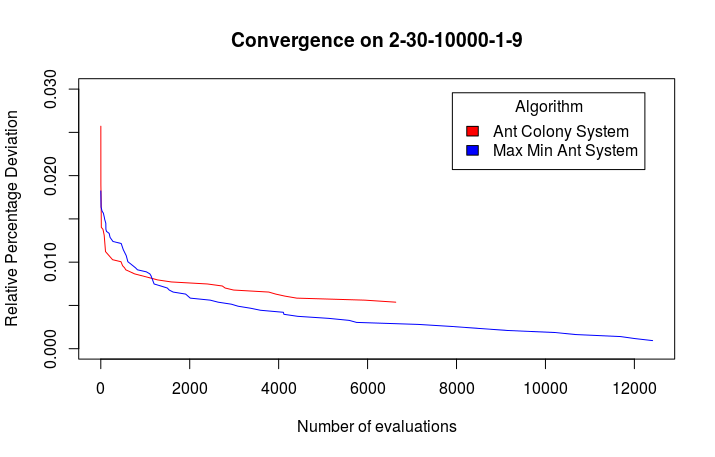
\includegraphics[scale=0.5]{conv-2-30}
    \caption{Convergence on 2-30-10000-1-9}
    \label{fig:conv1}
\end{figure}

\begin{figure}
    \centering
        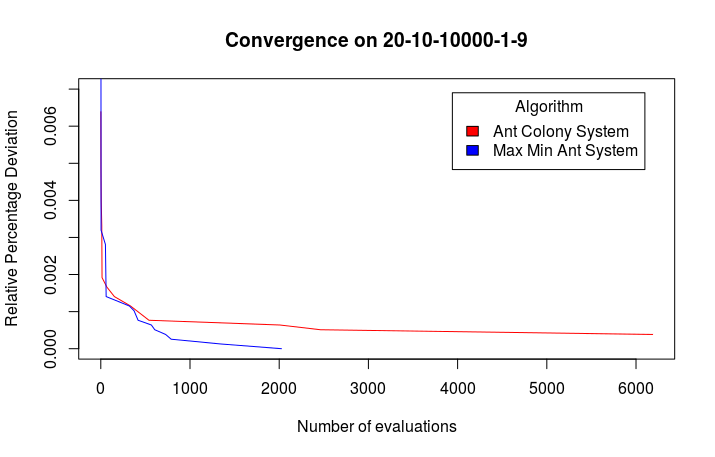
\includegraphics[scale=0.5]{conv-20-10}
    \caption{Convergence on 20-10-10000-1-9}
    \label{fig:conv2}
\end{figure}

\section{Local search}

To improve the result of the algorithm, it is possible to execute a local search.
In this project, the local search is applied to the Max Min Ant System Algorithm.

\subsection{Principle}

The principle of a local search is to perform few modifications on a solution.
These modifications create new solutions which are calle neighbours.
These solution can be evaluated and hopefully replace the best solution found so far.
Once a better solution is found, the process can be executed again on this new solution.

\subsection{Application to the Closest String Problem}

The neighbourhood chosen is the set of solutions that differs with only one character from the initial solution.
The local search algorihtm implemented iterates over all the neighbours and select the best one. (best improvement rule)
If the best neighbour is better than the best solution found so far, the process is restarted with this new solution. \newline

To implement the local search efficiently, the evaluation of the solution needs to be fast.
In this problem, this is possible by keeping the distances of each strings in the memory and comparing the new character of the solution to the previous one to update the distance ifnecessary.
However, the execution of the local search after each improvement remains slow.
For this reason, the local search is only applied at the end of the algorithm, on the best solution found.

\subsection{Comparisons with the local search}

The Max Min variant with the local search executed at the and has been tested with 10 runs on each instances, the the same seed used for the previous tests. \newline

The table in \ref{app:rpd}, contains the relative percentage deviations from the upper bound.
In the table \ref{app:rpdsum}, we can see that the local search improves the results of the Max Min algorithm.
Once again, it is possible to execute a wilcoxon test to see if there is a statistically sifgnificant difference between the solution qualities of the Max Min algorithm and the Max Min + loca search. \newline

With a significance level equal to 0.05, the Wilcoxon test returns a p-value equal to 0.693.
So it is not possible to conclude that there is a significant difference between the solution qualities.
However, it is obvious that the local search cannot return worst result.
It can be preferable to use the local search if this step does not take too much time. \newline

To finish, it is also possible to apply the Wilcoxon test to compare the results between the solution qualities of the Max Min + local search and the Ant Colony System algorithm.
With the same significance level, the p-value returned is equal to 0.130, which does not give another conclusion.

\subsection{Parameter settings with the local search}

The parameter settings of the Max Min Ant System has been re-executed after the addition of the local search.
However, as said before, the local search is only applied at the end of the algorithm.
Then, the local search does not change the best tuning.
Nevertheless, we can observe that the bigger the deviation to the upper bound is, the more efficient the local search is.
Thus, if the tuning is not efficient, the local search can still make the result interesting.


\section*{Conclusion}

To conclude, we can see that the ant colony algorithms can be very efficient on combinatorial optimization problems like the Closest String one.
The comparison of the two algorithms shows that with good parameter settings, the different algorithms are very close in terms of quality.
However, the convergences comparison shows that they do not have exactly the same behaviours.
Thus some algorithms could be more interesting to obtain very high quality fast and others could be interesting to get very close to the optimal solution.
One of the main difficulty of the ant colony algorithms remains the parameter settings.
Multiple techniques have been used but the help of automatic parameter settings algorithms might be usefull to improve the results of the algorithms.

\section{Appendices}

\subsection{Appendix A}

The table bellow shows the relative percentage deviations of the solutions' means from the upper bound for all the algorithms implemented.
MMAS means Max Min Ant System, ACS means Ant Colony System and MMAS LS corresponds to The Max Min Ant System with the local search.\\

\label{app:rpd}

\begin{tabular}{c|c|c|c}
instance & MMAS rpd & ACS rpd & MMAS LS rpd \\
\hline
20-10-10000-1-9 & 0.005 & 0.051 & 0 \\
20-20-10000-1-7 & 0.134 & 0.220 & 0.119 \\
20-30-10000-1-5 & 0.150 & 0.211 & 0.139 \\
20-40-10000-1-3 & 0.209 & 0.266 & 0.183 \\
20-50-10000-1-1 & 0.308 & 0.357 & 0.294 \\
2-30-10000-1-9 & 0.327 & 0.605 & 0.281 \\
2-30-10000-2-8 & 0.356 & 0.611 & 0.304 \\
2-40-10000-1-7 & 0.766 & 1.034 & 0.755 \\
2-40-10000-2-6 & 0.546 & 0.724 & 0.480 \\
2-50-10000-1-5 & 0.583 & 0.810 & 0.607 \\
2-50-10000-2-4 & 0.696 & 0.914 & 0.653 \\
4-20-10000-1-2 & 0.208 & 0.396 & 0.174 \\
4-20-10000-2-3 & 0.073 & 0.109 & 0.081 \\
4-30-10000-1-1 & 0.205 & 0.334 & 0.199 \\
4-30-10000-2-0 & 0.198 & 0.262 & 0.180 \\
4-40-10000-1-9 & 0.394 & 0.498 & 0.375 \\
4-40-10000-2-8 & 0.130 & 0.164 & 0.140 \\
4-50-10000-1-7 & 0.419 & 0.542 & 0.400 \\
4-50-10000-2-6 & 0.040 & 0.056 & 0.040 \\
\end{tabular}

\subsection{Appendix B}

The table bellow shows the maximum, the minimum, the mean and the standard deviation of the relative percentage deviations for each algorithms.\\

\label{app:rpdsum}

\begin{tabular}{c|c|c|c|c}
    algorithm & min & max & mean & sd \\
    \hline
    MMAS & 0.005 & 0.766 & 0.303 & 0.219 \\
    ACS & 0.051 & 1.034 & 0.430  & 0.292 \\
    MMAS + LS & 0 & 0.755 & 0.284 & 0.213
\end{tabular}\\

\begin{thebibliography}{2}

\bibitem{aco_csp} Simone Faro and Elisa Pappalardo.
Ant-CSP: An Ant Colony Optimization Algorithm for the Closest String Problem, pages 370-381.
Springer Berlin
Heidelberg, Berlin, Heidelberg, 2010.

\end{thebibliography}

\end{document}
